\documentclass[letterpaper]{article}
\usepackage{natbib,alifeconf}
\usepackage{amsmath,amssymb}
\usepackage{graphicx,booktabs,microtype,float}
\usepackage[hidelinks]{hyperref}
\graphicspath{{figures/}}
\setlength{\textfloatsep}{7pt plus 1pt minus 1pt}
\setlength{\floatsep}{6pt plus 1pt minus 1pt}
\setlength{\dbltextfloatsep}{6pt plus 1pt minus 1pt}
\setlength{\abovecaptionskip}{3pt}
\setlength{\belowcaptionskip}{0pt}
\setlength{\titlebox}{1.72in}

\title{Winnower: Detecting Periodic Domains in Cellular Automata}
\author{Author information to be added for submission}

\begin{document}
\maketitle

\noindent\textbf{Motivation.}
Cellular automata often form broad periodic domains together with defects, particles, and interfaces. Those domains are visually obvious in many rules, but choosing \emph{which} global period best explains a finite spacetime is less obvious. We introduce \emph{Winnower}, a fast selector for that task. Each candidate period/shift pair is treated as a model class, fit to its nearest periodic background by majority vote on orbit classes, and scored with a Bernoulli normalized maximum likelihood (NML) criterion.

\begin{figure}[H]
    \centering
    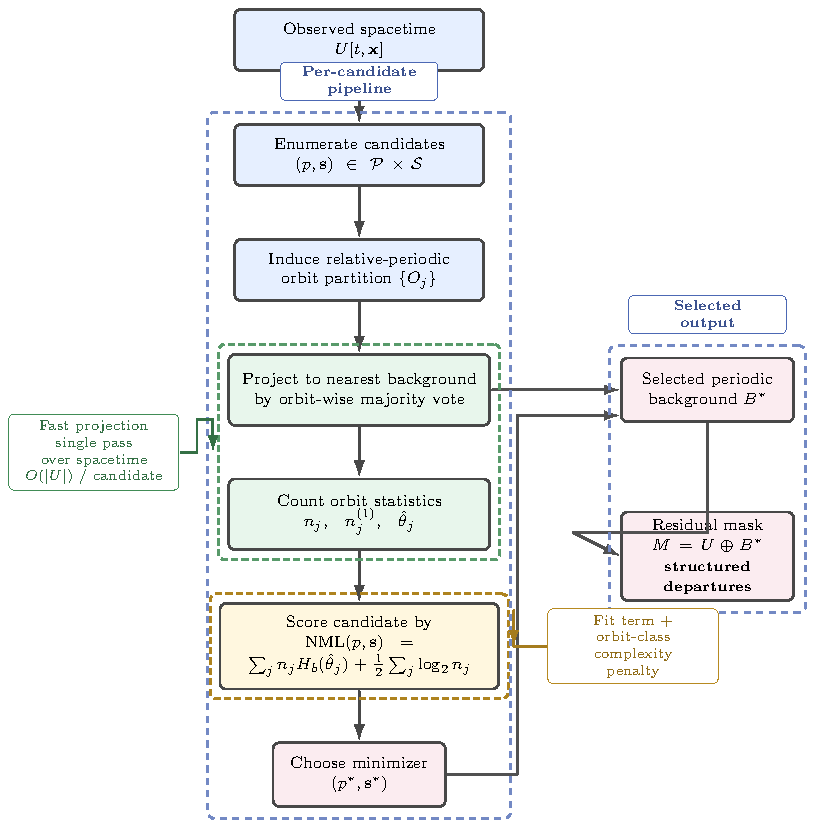
\includegraphics[width=1.02\columnwidth]{algorithm_detailed_tikz.pdf}
    \caption{Winnower algorithm sketch. The layout now uses external highlight panels for the fast-projection claim and the fit-plus-penalty score, with straight orthogonal connectors and enlarged vertical spacing so the annotation panels stay close to the pipeline without crossing it.}
    \label{fig:algorithm}
    \vspace{-0.35em}
\end{figure}

\noindent\textbf{Method.}
For a candidate period $p$ and shift $\mathbf{s}$, Winnower uses the translation $(t,\mathbf{x})\mapsto (t+p,\mathbf{x}+\mathbf{s})$ to partition spacetime into orbit classes. Each orbit contributes one background bit, chosen by majority vote, so fitting is linear in the number of observed sites. The NML score combines Bernoulli data fit and a complexity penalty. That penalty matters because along velocity-matched divisibility chains, larger templates can only improve raw residual and raw likelihood.

\noindent\textbf{Findings.}
Across the current 1D, 2D, and 3D case studies, the selected period either stabilizes immediately or changes only a small number of times before locking. Rule~54 stabilizes at period~4 from the first measured horizon; Rule~110 passes through a short transient before locking at period~4 under the period-first selector; S24/B11 in 2D later shifts from period~1 to period~2; and the tested 3D diamoeba rule remains at period~1 throughout the observed range. After locking, the winning margin grows rather than shrinks, which matches the model-selection picture behind the full paper. The penalty also changes the selector qualitatively: on 105 nontrivial Life-like rules at $T=100$, Bernoulli NLL without the penalty chooses the largest tested period in every case, whereas Bernoulli NML selects period~1 for 97 rules, period~2 for 7, and period~8 for 1.

\begin{figure*}[!t]
    \centering
    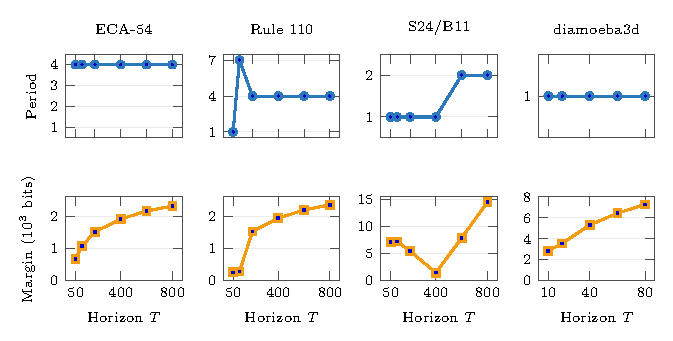
\includegraphics[width=0.86\textwidth]{stabilization_summary_tikz.pdf}
    \caption{Representative stabilization patterns. The top row shows selected period versus horizon; the bottom row shows the winning margin in bits. Some rules lock immediately (ECA-54, diamoeba3d), while others make a small number of transitions before locking (ECA-110, S24/B11).}
    \label{fig:stabilization}
\end{figure*}

\noindent\textbf{Why this matters for ALIFE.}
Winnower is deliberately modest. It does not replace local causal-state reconstruction, and it does not claim that the selected period is always a physicist's ``true'' background period. Instead it provides a global front end: a compact domain hypothesis, a residual mask, and a complexity-penalized way to compare periodic explanations across many rules. That makes it useful for large surveys and for follow-on analysis of particles, defects, and coherent structures.

\newpage
\small
\begin{thebibliography}{9}
\bibitem[Crutchfield and Hanson, 1997]{crutchfield1997}
Crutchfield, J.~P. and Hanson, J.~E. (1997). Computational mechanics of cellular automata: An example. \emph{Physica D}, 103:169--189.
\bibitem[Gr{\"u}nwald, 2007]{grunwald2007}
Gr{\"u}nwald, P. (2007). \emph{The Minimum Description Length Principle}. MIT Press.
\bibitem[Hanson and Crutchfield, 1992]{hanson1992}
Hanson, J.~E. and Crutchfield, J.~P. (1992). The attractor-basin portrait of a cellular automaton. \emph{Journal of Statistical Physics}, 66:1415--1462.
\bibitem[Rupe and Crutchfield, 2018]{rupe2018}
Rupe, A. and Crutchfield, J.~P. (2018). Local causal states and discrete coherent structures. \emph{Chaos}, 28:075312.
\bibitem[Shalizi et~al., 2006]{shalizi2006}
Shalizi, C.~R., Haslinger, R., Rouquier, J.-B., Klinkner, K.~L., and Moore, C. (2006). Automatic filters for the detection of coherent structure in spatiotemporal systems. \emph{Physical Review E}, 73:036104.
\bibitem[Shtarkov, 1987]{shtarkov1987}
Shtarkov, Y. (1987). Universal sequential coding of single messages. \emph{Problems of Information Transmission}, 23:3--17.
\end{thebibliography}

\end{document}
